% AER E 361 Mission Report Template
% Spring 2023
% Template created by Yiqi Liang and Professor Matthew Nelson

% Document Configuration DO NOT CHANGE
\documentclass[12 pt]{article}
% --------------------LaTeX Packages---------------------------------
% The following are packages that are used in this report.
% DO NOT CHANGE ANY OF THE FOLLOWING OR YOUR REPORT WILL NOT COMPILE
% -------------------------------------------------------------------

\usepackage{hyperref}
\usepackage{parskip}
\usepackage{titlesec}
\usepackage{titling}
\usepackage{graphicx}
\usepackage{graphviz}
\usepackage[T1]{fontenc}
\usepackage{titlesec, blindtext, color} %for LessIsMore style
\usepackage{tcolorbox} %for references box
\usepackage[hmargin=1in,vmargin=1in]{geometry} % use 1 inch margins
\usepackage{float}
\usepackage{tikz}
\usepackage{svg} % Allows for SVG Vector graphics
\usepackage{textcomp, gensymb} %for degree symbol
\hypersetup{
	colorlinks=true,
	linkcolor=blue,
	urlcolor=cyan,
}
\usepackage{biblatex}
\addbibresource{lab-report-bib.bib}
\usepackage{amsmath}
\usepackage{listings}
\usepackage{multicol}
\usepackage{array}

\usepackage{hologo} %KYR: for \BibTeX
%\usepackage{algpseudocode}
%\usepackage{algorithm}
% This configures items for code listings in the document
\usepackage{xcolor}

\usepackage{fancyhdr} % Headers/Footers
\usepackage{siunitx} % SI units
\usepackage{csquotes} % Display Quote
\usepackage{microtype} % Better line breaks

\definecolor{commentsColor}{rgb}{0.497495, 0.497587, 0.497464}
\definecolor{keywordsColor}{rgb}{0.000000, 0.000000, 0.635294}
\definecolor{stringColor}{rgb}{0.558215, 0.000000, 0.135316}
\definecolor{mygreen}{rgb}{0,0.6,0}
\definecolor{mygray}{rgb}{0.5,0.5,0.5}
\definecolor{mymauve}{rgb}{0.58,0,0.82}

\lstdefinestyle{customc}{
  belowcaptionskip=1\baselineskip,
  breaklines=true,
  frame=L,
  xleftmargin=\parindent,
  language=C,
  showstringspaces=false,
  basicstyle=\footnotesize\ttfamily,
  keywordstyle=\bfseries\color{green!40!black},
  commentstyle=\itshape\color{purple!40!black},
  identifierstyle=\color{blue},
  stringstyle=\color{orange},
 }

 \lstset{ %
  backgroundcolor=\color{white},   % choose the background color; you must add \usepackage{color} or \usepackage{xcolor}
  basicstyle=\footnotesize,        % the size of the fonts that are used for the code
  breakatwhitespace=false,         % sets if automatic breaks should only happen at whitespace
  breaklines=true,                 % sets automatic line breaking
  captionpos=b,                    % sets the caption-position to bottom
  commentstyle=\color{commentsColor}\textit,    % comment style
  deletekeywords={...},            % if you want to delete keywords from the given language
  escapeinside={\%*}{*)},          % if you want to add LaTeX within your code
  extendedchars=true,              % lets you use non-ASCII characters; for 8-bits encodings only, does not work with UTF-8
  frame=tb,	                   	   % adds a frame around the code
  keepspaces=true,                 % keeps spaces in text, useful for keeping indentation of code (possibly needs columns=flexible)
  keywordstyle=\color{keywordsColor}\bfseries,       % keyword style
  language=Python,                 % the language of the code (can be overrided per snippet)
  otherkeywords={*,...},           % if you want to add more keywords to the set
  numbers=left,                    % where to put the line-numbers; possible values are (none, left, right)
  numbersep=8pt,                   % how far the line-numbers are from the code
  numberstyle=\tiny\color{commentsColor}, % the style that is used for the line-numbers
  rulecolor=\color{black},         % if not set, the frame-color may be changed on line-breaks within not-black text (e.g. comments (green here))
  showspaces=false,                % show spaces everywhere adding particular underscores; it overrides 'showstringspaces'
  showstringspaces=false,          % underline spaces within strings only
  showtabs=false,                  % show tabs within strings adding particular underscores
  stepnumber=1,                    % the step between two line-numbers. If it's 1, each line will be numbered
  stringstyle=\color{stringColor}, % string literal style
  tabsize=2,	                   % sets default tabsize to 2 spaces
  title=\lstname,                  % show the filename of files included with \lstinputlisting; also try caption instead of title
  columns=fixed                    % Using fixed column width (for e.g. nice alignment)
}

\lstdefinestyle{customasm}{
  belowcaptionskip=1\baselineskip,
  frame=L,
  xleftmargin=\parindent,
  language=[x86masm]Assembler,
  basicstyle=\footnotesize\ttfamily,
  commentstyle=\itshape\color{purple!40!black},
}

\lstset{escapechar=@,style=customc}

\titlelabel{\thetitle.\quad}

% From here on out you can start editing your document
\newcommand{\subtitle}[1]{%
  \posttitle{%
    \par\end{center}
    \begin{center}\LARGE#1\end{center}
    \vskip0.5em}%
}

\title{\textbf{Iowa State University
\\{\Large Aerospace Engineering}}}
\subtitle{AER E 322 Lab 7\\
		  Column Buckling}
\author{Matthew Mehrtens, Peter Mikolitis, and Natsuki Oda}

\newcommand{\etal}{\textit{et al}., }
\newcommand{\ie}{\textit{i}.\textit{e}., }
\newcommand{\eg}{\textit{e}.\textit{g}., }

% Define the headers and footers
\setlength{\headheight}{70.63135pt}
\geometry{head=70.63135pt, includehead=true, includefoot=true}
\pagestyle{fancy}
\fancyhead{}\fancyfoot{} % clears the headers/footers
\fancyhead[L]{\textbf{AER E 322}}
\fancyhead[C]{\textbf{Aerospace Structures Laboratory Summary}\\
			  \textbf{Lab 7 Column Buckling}\\
			  Section 4 Group 2\\
			  Matthew Mehrtens, Peter Mikolitis, and Natsuki Oda\\
			  \today}
\fancyhead[R]{\textbf{Spring 2023}}
\fancyfoot[C]{\thepage}

\begin{document}
\maketitle
\tableofcontents
\section{Introduction} \label{introduction}
In this lab, we studied column buckling by using the Instron machines to apply a compressive load to five different column specimens. The columns varied in shape/dimensions, material, length, and ``end-configuration''. We tested a cylindrical and rectangular aluminum column and three cylindrical steel columns. By varying the properties of the columns, we were able to make connections between the theoretical or calculated material properties and the physical behavior of columns. In doing so, we gained a better insight into static column design and analysis.

\section{Objectives} \label{objectives}
\begin{itemize}
	\item Accurately predict the force at which the sample will buckle
	\item Visually observe the column buckling and record the force at which buckling first occured
	\item Use the analysis of observations from the lab to design a new column
\end{itemize}

\section{Hypothesis} \label{hypothesis}
For the rectangular specimen, we expected the column to buckle about the axis with the lowest moment of inertia, \ie the axis with the least resistance to bending. We also expected the cylindrical aluminum column and the one-pivot-one-fixed cylindrical steel column to have the least perceptible ``jolt'' due to their relatively low slenderness ratios.

\section{Work Assignments} \label{work_assignments}
Refer to Table \ref{table:work_assignments} for the distribution of work during this lab.

\begin{table}[!htbp]
\caption{Work assignments for AER E 322 Lab 7.}
\begin{center}
	\begin{tabular}{| c | c | c | c |}
		\hline
		\multicolumn{1}{| c |}{\textbf{Task}} & \textbf{Matthew} & \textbf{Peter} & \textbf{Natsuki} \\
		\hline
		\multicolumn{4}{| c |}{\textit{Lab Work}} \\
		\hline
		Data Recording & X & X & X \\
		\hline
		Exp. Setup & X & X & X \\
		\hline
		Exp. Work & X & X & X \\
		\hline
		Exp. Clean-Up & X & X & X \\
		\hline
		\multicolumn{4}{| c |}{\textit{Report}} \\
		\hline
		Introduction & X & X & \\
		\hline
		Objectives & & X & \\
		\hline
		Hypothesis & & X & \\
		\hline
		Materials & & & X \\
		\hline
		Apparatus & & & X \\
		\hline
		Procedures & & & X \\
		\hline
		Data & X & & \\
		\hline
		Analysis & X & X & X \\
		\hline
		Conclusion & X & X & \\
		\hline
		Editing & & & \\
		\hline
	\end{tabular}
\end{center}
\label{table:work_assignments}
\end{table}

\section{Materials} \label{materials}
\begin{itemize}
	\item Five metal column specimens with specifications defined in \ref{tbl:column_specs}
	\item Instron machine (see Figures \ref{fig:instron_1} and \ref{fig:instron_2})
	\item Socket to fix the ends of the specimens in a pivot configuration (see Figure \ref{fig:socket})
	\item Ruler to measure the length of the specimen 
\end{itemize}

\begin{table}[!htbp]
\caption{The five column buckling test configurations.}
\begin{center}
	\begin{tabular}{|c|c|c|c|c|}
		\hline
		Specimen ID&Material&Cross-Section [\unit{in.}]&Length [\unit{in.}]&End Condition\\
		\hline
		I&aluminum&$\frac{3}{8}$ dia.&\num{30}&both pivot (round)\\
		\hline
		II&aluminum&\numproduct{0.25x1}&\num{30}&both pivot (round)\\
		\hline
		III&steel&$\frac{1}{4}$ dia.&\num{30}&both pivot (round)\\
		\hline
		IV&steel&$\frac{1}{4}$ dia.&\num{24}&both pivot (round)\\
		\hline
		V&steel&$\frac{1}{4}$ dia.&\num{27.5} (\num{30} original)&one pivot, one fixed\\
		\hline
	\end{tabular}
\end{center}
\label{tbl:column_specs}
\end{table}

\section{Apparatus} \label{apparatus}
\begin{figure}[htbp]
    \centering
    \begin{minipage}{0.45\textwidth}
        \centering
		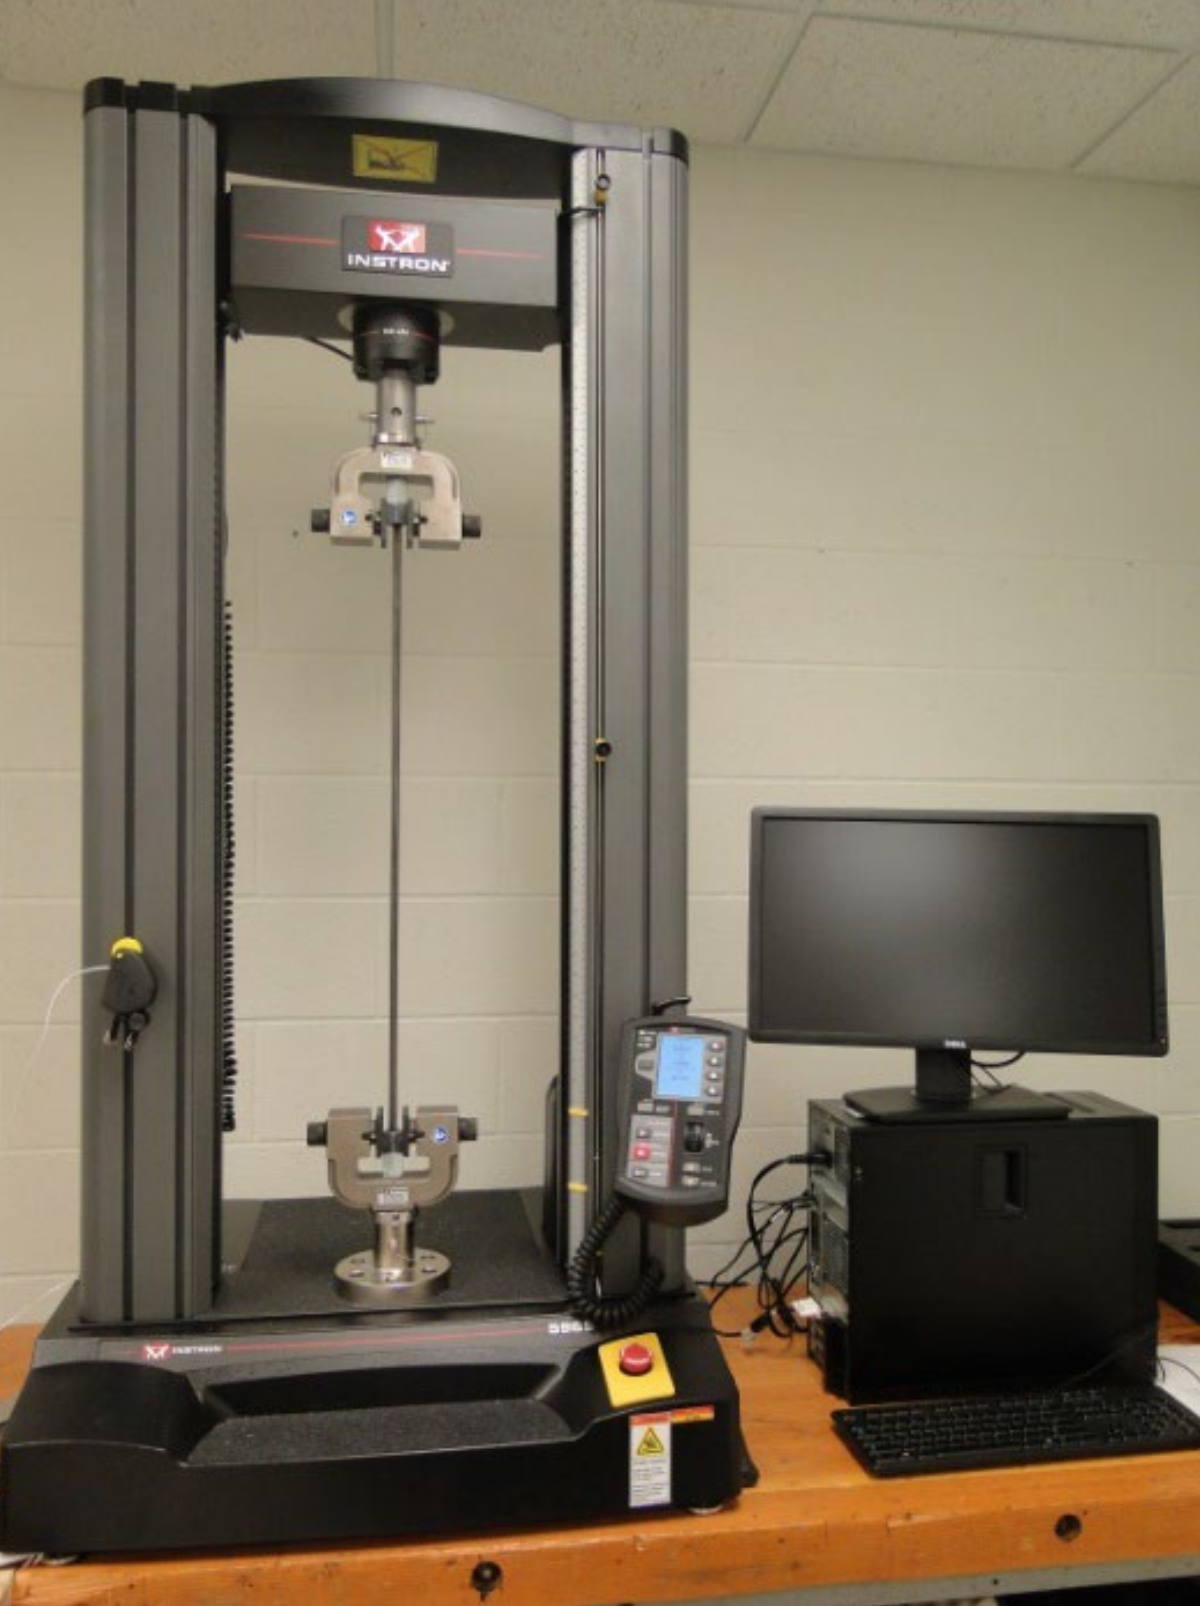
\includegraphics[width=1.0\textwidth]{images/instron_1}
		\caption{The Instron loaded with a metal column specimen.}
		\label{fig:instron_1}
    \end{minipage}\hfill
    \begin{minipage}{0.45\textwidth}
        \centering
		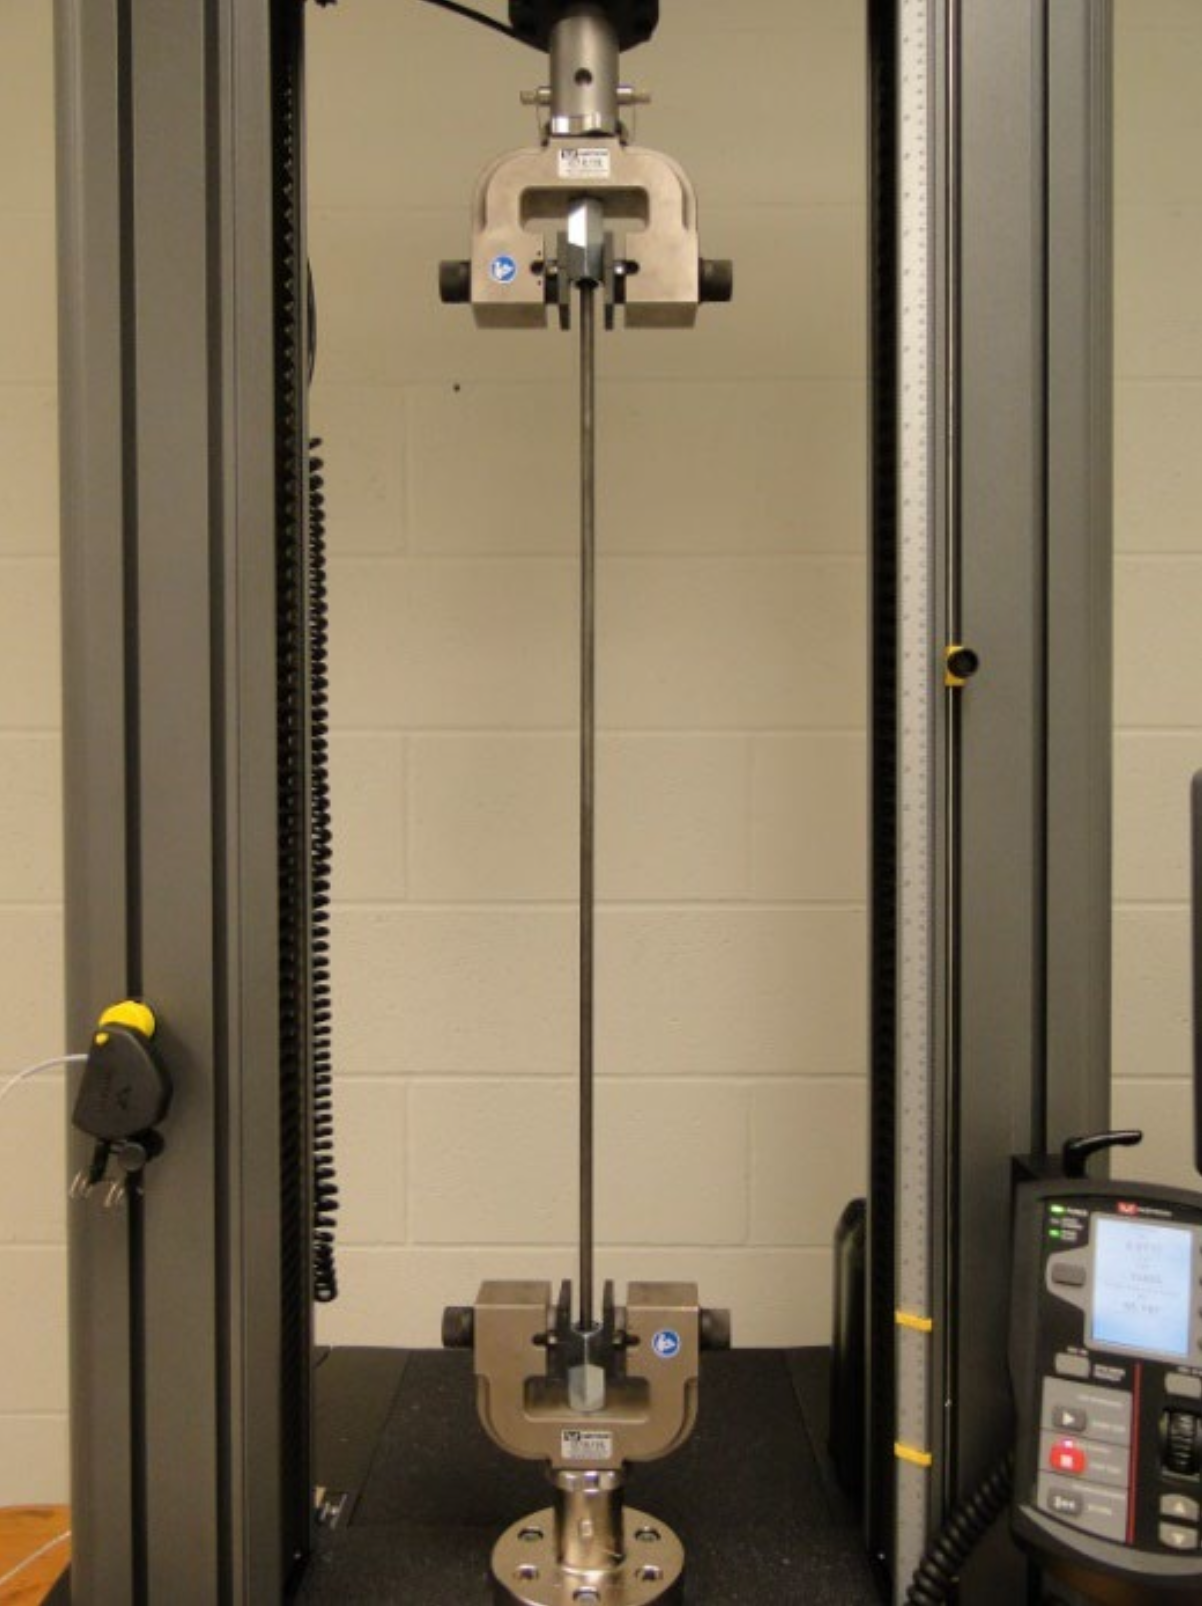
\includegraphics[width=1.0\textwidth]{images/instron_2}
		\caption{The Instron configured for a column buckling test.}
		\label{fig:instron_2}
    \end{minipage}
\end{figure}

\begin{figure}[htbp]
	\centering
	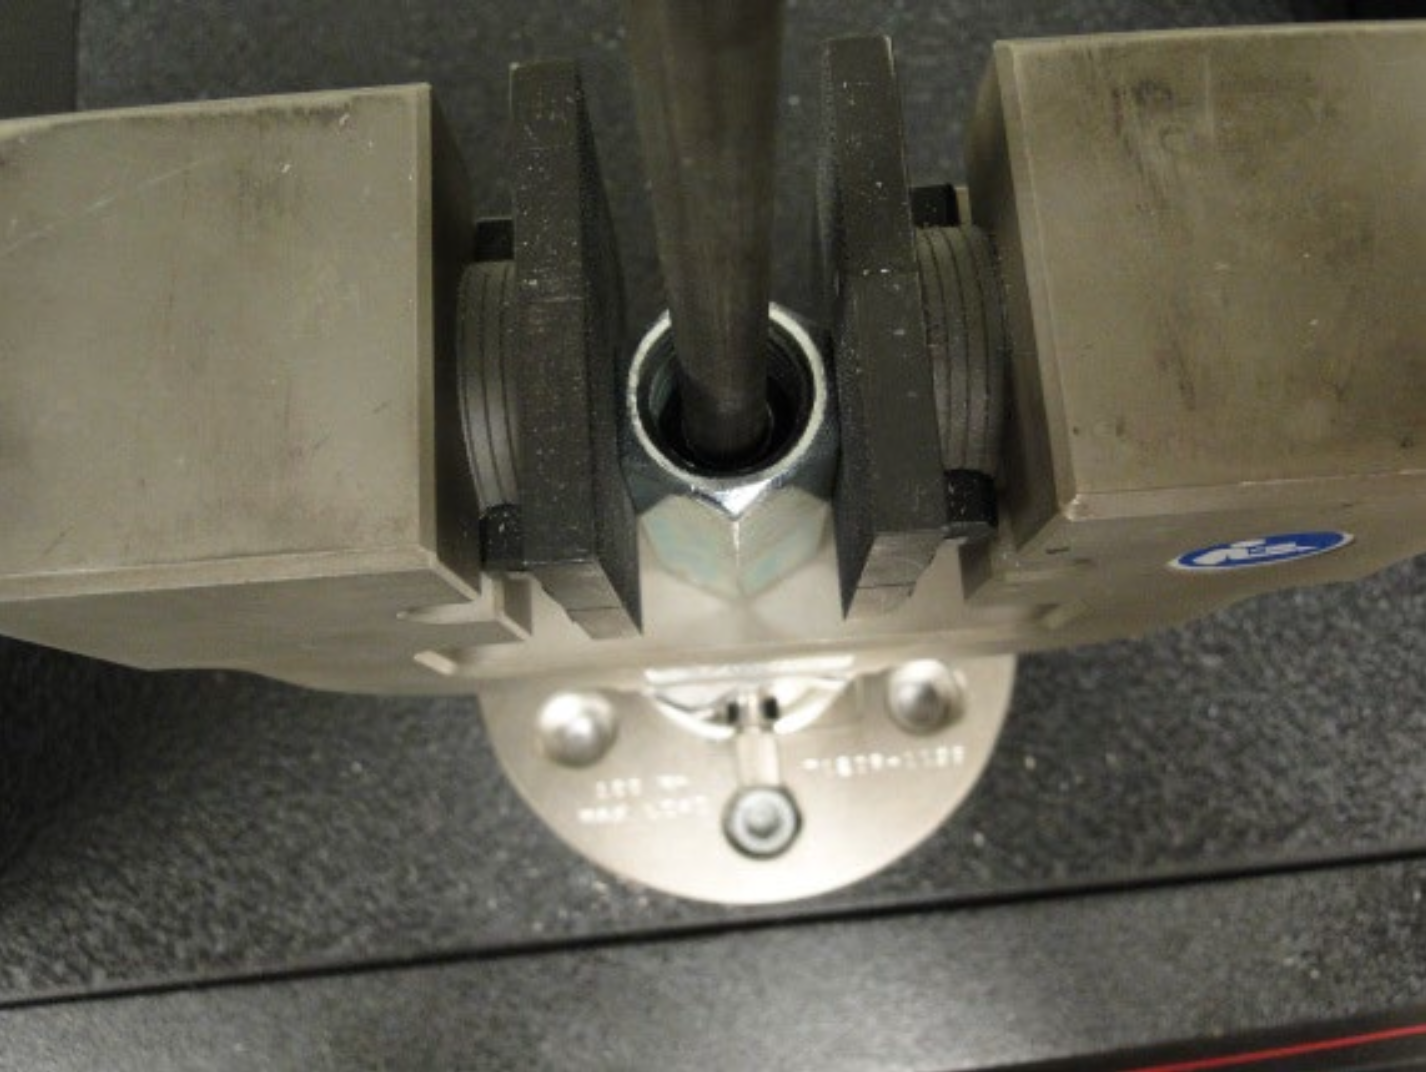
\includegraphics[width=4in]{images/socket}
	\caption{A close-up of the socket used to hold the specimens in the Instron machine.}
	\label{fig:socket}
\end{figure}

\section{Procedures} \label{procedures}
Insert the specimen into the Instron. While the specimen is in the socket, but still unloaded, zero the Instron to reset all the measurements. Using the fine adjustment knob, decrease the gaps between the specimen ends and the sockets until the specimen is loaded with \qty{5}{lb}. Record the distance between the sockets or between the socket and the grip.

Visually align the column with a vertical marker behind the column. Increase the compressive force with the fine adjustment knob at a rate of one click per second. Once the specimen ``jolts'' or buckles away from the visual marker, note and record the current force. Unload the specimen. Repeat this whole procedure for all five specimen.

\section{Data} \label{data}
Data collected from the experiment is tabulated in Table \ref{tbl:data}.

\begin{table}[!htbp]
\caption{Data collected from the lab. Specimen one through three were tested twice whereas specimens four through five were tested three times. $P_\text{cr}$ is the theoretical critical load.}
\begin{center}
	\begin{tabular}{|c|c|c|c|c|}
		\hline
		Specimen ID&Length [\unit{in}]&$P_\text{cr,avg}$ [\unit{in}]&$P_\text{cr}$ [\unit{in}]&Error\\
		\hline
		I&\num{30}&\num{-133}&\num{-106.5}&\qty{24.9}{\percent}\\
		\hline
		II&\num{29.5}&\num{-126}&\num{-147.7}&\qty{14.7}{\percent}\\
		\hline
		III&\num{30}&\num{-54.8}&\num{-60.98}&\qty{10.1}{\percent}\\
		\hline
		IV&\num{24}&\num{-91.7}&\num{-92.58}&\qty{0.915}{\percent}\\
		\hline
		V&\num{27.5}&\num{-102}&\num{-148.1}&\qty{31.4}{\percent}\\
		\hline
	\end{tabular}
\end{center}
\label{tbl:data}
\end{table}

\section{Analysis} \label{analysis}
% TODO

\section{Conclusion} \label{conclusion}
% TODO

\end{document}
